% !TEX root = ReviewDraft.tex



As we mentioned above,  the Bekenstein Hawking entropy formula should be viewed as the coarse-grained entropy formula for the black hole, since it increases under time evolution. This is clear when the black hole first forms and has not yet had time to emit Hawking radiation. 

Surprisingly there is also a gravitational formula for the von Neumann or fine-grained entropy  \cite{Ryu:2006bv,Hubeny:2007xt,Faulkner:2013ana,Engelhardt:2014gca}. It is also given by a formula that involves a generalized entropy, with an area plus the entropy of fields outside. The only difference is in the choice of the dividing surface. Roughly the idea is that we choose a surface such that the generalized entropy is minimized. This minimal value is the fine-grained entropy,   
\be \la{Appr}
 S \sim {\rm min} \left[ {{ \rm Area } \over 4 \GN} + S_{\rm outside} \right]  \ .
 \ee 
 
 \begin{figure}[t]
\begin{center}
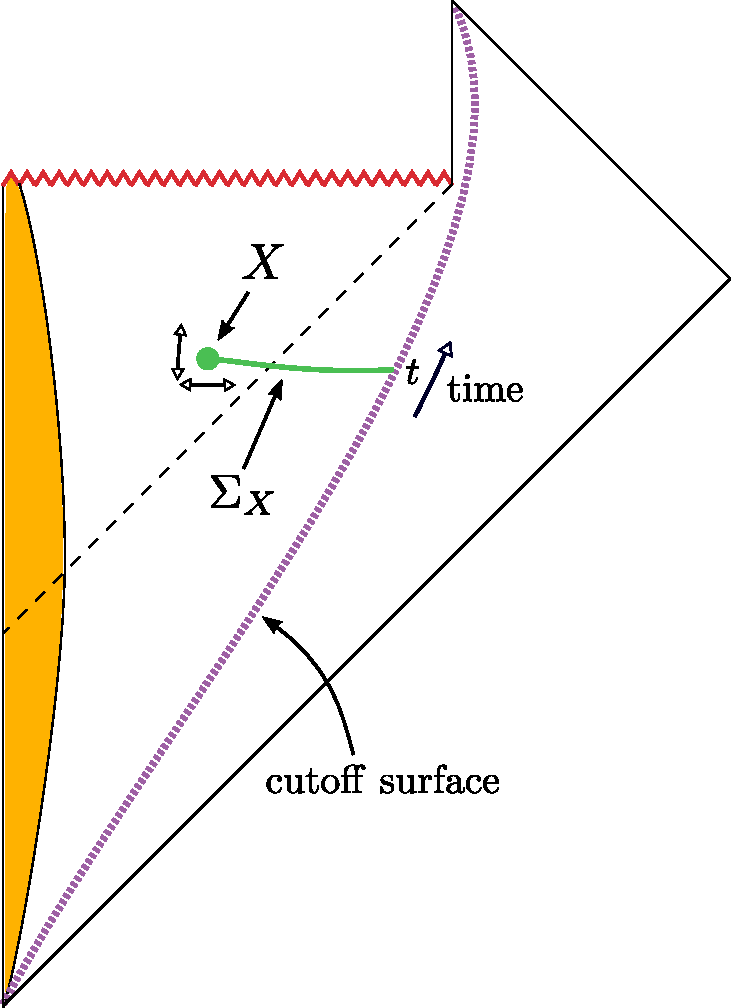
\includegraphics[scale=0.4]{figures/bhprocedure.pdf}
\caption{The procedure for finding the extremal surface for computing the time-dependent fine-grained entropy of black hole. Starting on the cutoff surface at a given time, the surface $X$ is deformed into the enclosed region until an extremum is found.
Recall that this diagram represents the radial and time direction, so a point on this diagram represents a sphere.  }
\label{bhprocedure}
\end{center}
\end{figure} 


 Now,  \nref{Appr} captures the spirit of the formula, but the precise formula is slightly more complicated. The reason is the following. A surface is a codimension-2 object. This means that it has two dimensions less than that of the full spacetime. In our case it is localized along one of the spatial dimensions and also in time. We are looking for a surface that     minimizes \nref{Appr} in the spatial direction but maximizes it in the time direction.  So we really should look for ``extremal surfaces'' by moving them both in space and in time. If there are many extremal surfaces we should find the global minimum. Another equivalent definition is the  following maxi-min construction  \cite{Wall:2012uf,Akers:2019lzs}.   First choose a spatial slice (a Cauchy slice) and find the minimal surface. Then find the maximum among all choices of the Cauchy slice.  Then a more precise version of the formula is 
 \cite{Ryu:2006bv,Hubeny:2007xt,Faulkner:2013ana,Engelhardt:2014gca} 
 \be \la{RT} 
\setlength\fboxsep{0.25cm}
\setlength\fboxrule{0.4pt}
 \boxed{ S= {\rm min}_X \left\{ {\rm ext}_X \left[ { {\rm Area}( X)  \over 4 G_N} + \Ssemi(\Sigma_X) \right] \right\}} \ ,
 \ee 
 where $X$ is a codimension-2 surface, $\Sigma_X$ is the region bounded by $X$ and the cutoff surface, and $\Ssemi(\Sigma_X)$ is the von Neumann entropy of the quantum fields on $\Sigma_X$ appearing in the semiclassical description, see figure \ref{bhprocedure}. The quantity in brackets is the generalized entropy,
 \be\la{sgendef}
 S_{\rm gen}(X) = { {\rm Area}( X)  \over 4 G_N} + \Ssemi(\Sigma_X) \ .
 \ee
 The idea is that we start from a surface outside the black hole and we can move it past the horizon into the interior to find the minimum. In particular this means that the answer depends on the geometry of the black hole interior. We can have black holes with similar exteriors but different interiors.  Such black holes will have different fine-grained entropies.
	It could happen that the surface can be shrunk completely in the interior of the black hole. In this case there is no area contribution. We will see this below in more detail. 
	
	\begin{figure}[t]
\begin{center}
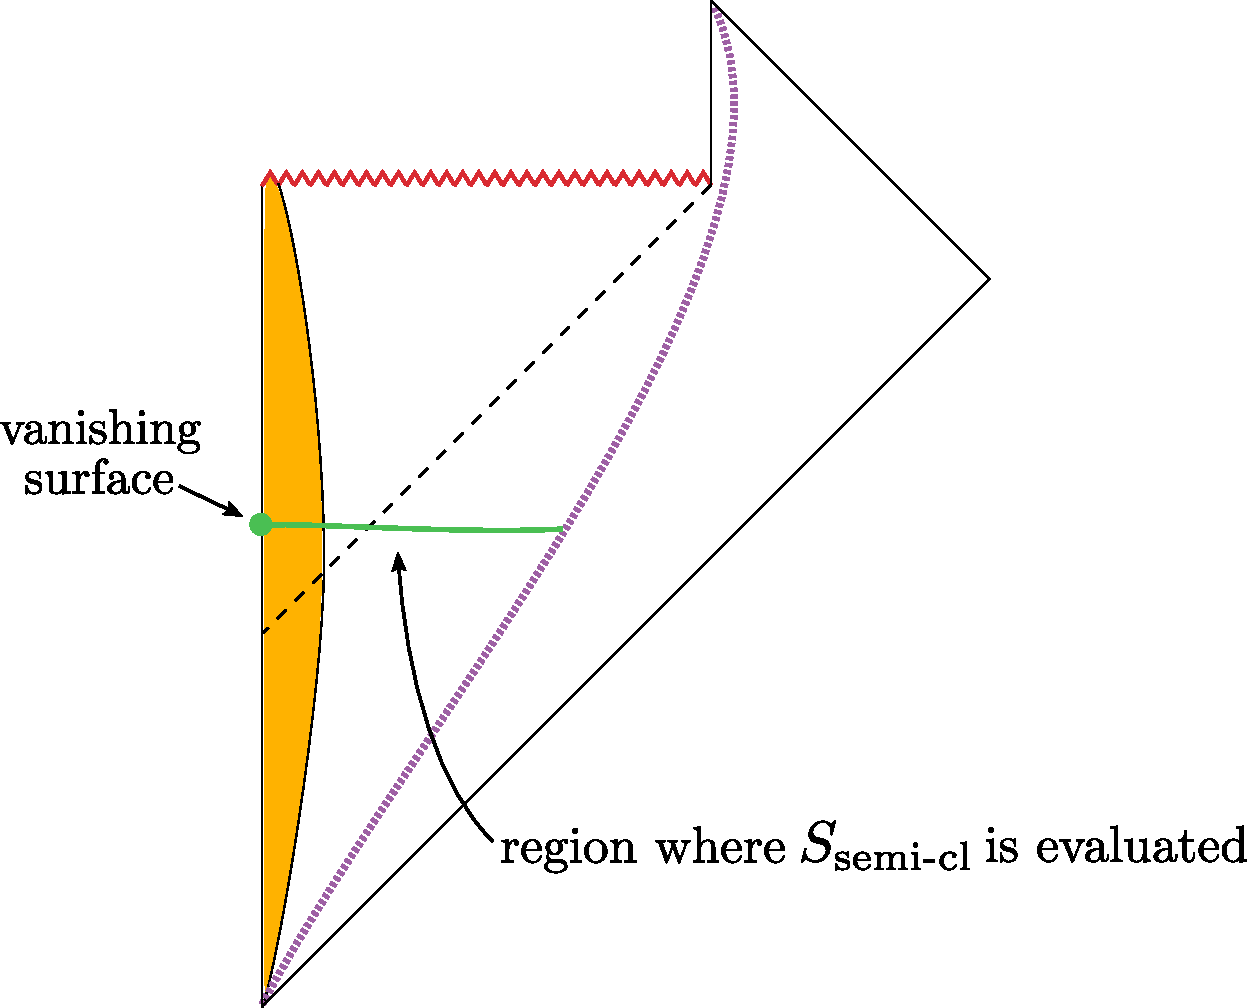
\includegraphics[scale=0.4]{figures/collapse-RT.pdf}
\caption{  \small The minimal surface for the black hole at early times shrinks down to zero size. We call this the vanishing surface. The generalized entropy reduces to the bulk entropy of the entire region enclosed by the cutoff surface. \label{CollapseRT}}

\end{center}
\end{figure}


\begin{itemize}
		
	\item
In the literature the surface that extremizes \nref{RT} is called the ``quantum extremal surface." 
Note that this is just a classical geometric surface in the spacetime. It is called ``quantum'' because the matter  contribution in \nref{RT} contains the entropy of the quantum fields. 
\item
	 This formula, \nref{RT},  can be derived by a method similar to the Gibbons Hawking method discussed in section \ref{ss:gibbonshawking} when there is a path integral prescription for the construction of the state  \cite{Lewkowycz:2013nqa,Faulkner:2013ana,Dong:2017xht}.
	 Something similar will be discussed in section \ref{replicas}.
	
	\end{itemize}



